% !TeX program = ptex2pdf -u -l
\documentclass[11pt,a4paper]{jsarticle}
%
\usepackage{amsmath,amssymb}
\usepackage{bm}
\usepackage[dvipdfmx]{graphicx}
\usepackage{ascmac}
\usepackage{atbegshi}
\usepackage[dvipdfmx]{geometry} % 追加: 余白を一時的に0にするため(dvipdfmx指定)
\usepackage{listings} % ソースコード表示のために追加
\usepackage{float}
\usepackage{hhline}
\usepackage{makecell} % セル内で明示改行(\\)を使うための最小変更
\usepackage{tcolorbox}
\newtcbox{\code}[1][]{
  colback=gray!10!white,
  colframe=gray!20!white,
  boxrule=0.5pt,
  left=2pt,right=2pt,top=1pt,bottom=1pt,
  box align=base,
  fontupper=\ttfamily
}
% 簡易コード表示用マクロ(本文中で\textttt{...}を使えるようにする)
\newcommand{\textttt}[1]{\texttt{#1}}
%ここからソースコードの表示に関する設定
\lstset{
  basicstyle={\ttfamily},
  identifierstyle={\small},
  commentstyle={\small\itshape},
  keywordstyle={\small\bfseries},
  ndkeywordstyle={\small},
  stringstyle={\small\ttfamily},
  frame={tb},
  breaklines=true,
  columns=[l]{fullflexible},
  numbers=left,
  xrightmargin=0zw,
  xleftmargin=3zw,
  numberstyle={\scriptsize},
  stepnumber=1,
  numbersep=1zw,
  lineskip=-0.5ex
}
\renewcommand{\lstlistingname}{ソースコード} % キャプションを「ソースコード」に変更
%ここまでソースコードの表示に関する設定
\newcommand{\myPdfAuthor}{平田爽馬/HIRATA,Soma}
\newcommand{\myPdfTitle}{EMI計測実験}
\AtBeginShipoutFirst{\special{pdf:tounicode EUC-UCS2}} % pLaTeXの内部漢字コードがEUCの場合
\AtBeginDvi{\special{pdf:docinfo <<
 /Author   (\myPdfAuthor)
 /Title    (\myPdfTitle)>>}}
%
\setlength{\textwidth}{\fullwidth}
\setlength{\textheight}{40\baselineskip}
\addtolength{\textheight}{\topskip}
\setlength{\voffset}{-0.2in}
\setlength{\topmargin}{0pt}
\setlength{\headheight}{0pt}
\setlength{\headsep}{0pt}
%
\newcommand{\divergence}{\mathrm{div}\,}  %ダイバージェンス
\newcommand{\grad}{\mathrm{grad}\,}  %グラディエント
\newcommand{\rot}{\mathrm{rot}\,}  %ローテーション
%
\title{\myPdfTitle}
\author{5E25番 平田爽馬}
\date{}
\begin{document}
%\maketitle%タイトルを挿入したくない場合は,消す
%
%
\section{目的}
私たちの周りには,妨害を発生する可能性を持つ多くの電気機器が存在している.
それらは雷に伴うサージや電磁波,人体などからの静電気放電などといった電気機器以外のものからの妨害とともに,他のものへの干渉を引き起こす可能性がある.
今回は,その中でも電気機器からの妨害の放射(EMI,日本語で電磁干渉)を計測することで,その基本を理解し,電気機器などを設計する上で必要な考えを理解する.

\section{EMCとは何か}
EMCは,Electro Magnetic Compatibilityの略であり,日本語では電磁両立性,電磁環境両立性などとも呼ばれている.
この用語は,「機器やシステムの,その環境内のいかなるものに対しても許容できない妨害を与えることなく,その電磁環境内において満足に機能する能力」のような形で定義される.
簡単に言えば,機器がその動作によってその他のものに妨害を与えず,EMCが達成されているということになる.

\subsection{なぜEMCが必要か}
EMCが欠如しているということは,何らかの干渉が発生することを意味する.
多くの人は電話やラジオへの雑音の混入やテレビの画像の乱れなどを経験したことはあるが,これもEMCが不十分であることによるものである.
やや深刻なEMC問題の身近な例の1つとしては,携帯電話とペースメーカーとの干渉の可能性が挙げられる.
私たちの周りには妨害を発生する可能性を持つ多くの電気機器が存在しており,それらは雷に伴うサージや電磁波,人体などからの静電気放電などといった電気機器以外のものからの妨害とともに,他のものへの干渉を引き起こす可能性を持っている.
このような干渉現象の例としては,表\ref{table1}に示すようなものが挙げられる.

\begin{table}[H]
\centering
\caption{干渉の例}
\label{table1}
\begin{tabular}{l|l} \hline
  \multicolumn{1}{c}{現象} & \multicolumn{1}{|c}{原因の例} \\ \hhline{=|=}
  ラジオやオーディオの雑音 & 電磁波,電源からの伝導性雑音 \\ \hline
  テレビの画像の乱れ & 電磁波,低周波磁界,電源からの伝導性雑音 \\ \hline
  テレビのゴースト & ビルからの放送波の反射 \\ \hline
  \makecell[l]{コンピュータや\\その他の電子機器の誤動作} & \makecell[l]{電磁波,電源からの伝導性雑音,\\静電気放電,サージ,電源電圧変動} \\ \hline
  照明のちらつき(フリッカ) & 電源電圧変動 \\ \hline
  \makecell[l]{変圧器の加熱,力率補償用コンデンサや\\雑音防止用コンデンサの破損} & 電源高調波電流 \\ \hline
  生体への影響 & 電磁波,低周波磁界  \\ \hline
\end{tabular}
\end{table}

\subsection{エミッションとイミュニティ}
機器からの妨害の放射(つまり,加害者としての振る舞い)は,エミッションと呼ばれる.
これは,EMI(Electro Magnetic Interface:電磁干渉)と呼ばれることもある.
また,妨害に関する耐性,すなわち妨害の受けにくさの程度はイミュニティと呼ばれる.
これは,その逆の妨害の受けやすさの程度を示す.
サセプティビリティ,あるいはEMS(Electro Magnetic Susceptibility:電磁感受性)という言葉で呼ばれることもある.
電気機器からのエミッションや電子機器への妨害の例を表\ref{table2}〜表\ref{table3}に示す.

\begin{figure}[H]
\centering
\includegraphics[width=75mm]{./fig/fig1.eps}
\caption{EMCの分類}
\label{fig1}
\end{figure}

\begin{figure}[H]
\centering
\includegraphics[width=70mm]{./fig/fig2.eps}
\caption{電子機器からの妨害の放射}
\label{fig2}
\end{figure}

\begin{table}[H]
\centering
\caption{エミッションの例}
\label{table2}
\begin{tabular}{l|l} \hline
  \multicolumn{1}{c}{発生源} & \multicolumn{1}{|c}{現象} \\ \hhline{=|=}
  \makecell[l]{放電灯,放電加工機,内燃機関の点火系,\\整流子電動機,接点の開閉,高圧線などの放電} & \makecell[l]{電磁波の放射} \\ \hline
  \makecell[l]{無線送信\\(放送,無線通信,レーダーなど)} & \makecell[l]{電磁波の意図的な放射,スプリアス} \\ \hline
  \makecell[l]{高周波エネルギー利用機器\\(高周波加熱装置,電子レンジなど)} & \makecell[l]{電磁波の放射} \\ \hline
  \makecell[l]{高周波信号利用機器\\(無線受信機,スペクトルアナライザなど)} & \makecell[l]{電磁波の放射} \\ \hline
  \makecell[l]{デジタル回路(情報技術機器,\\マイクロプロセッサ利用機器など)} & \makecell[l]{電磁波の放射,電源系統への高周波雑音や\\サージの注入,電源電圧変動の誘起(フリッカ)} \\ \hline
  \makecell[l]{交流電源(送電線,変圧器,電動機など)} & \makecell[l]{電源系統への雑音の注入,電源高調波電流} \\ \hline
\end{tabular}
\end{table}

\begin{figure}[H]
\centering
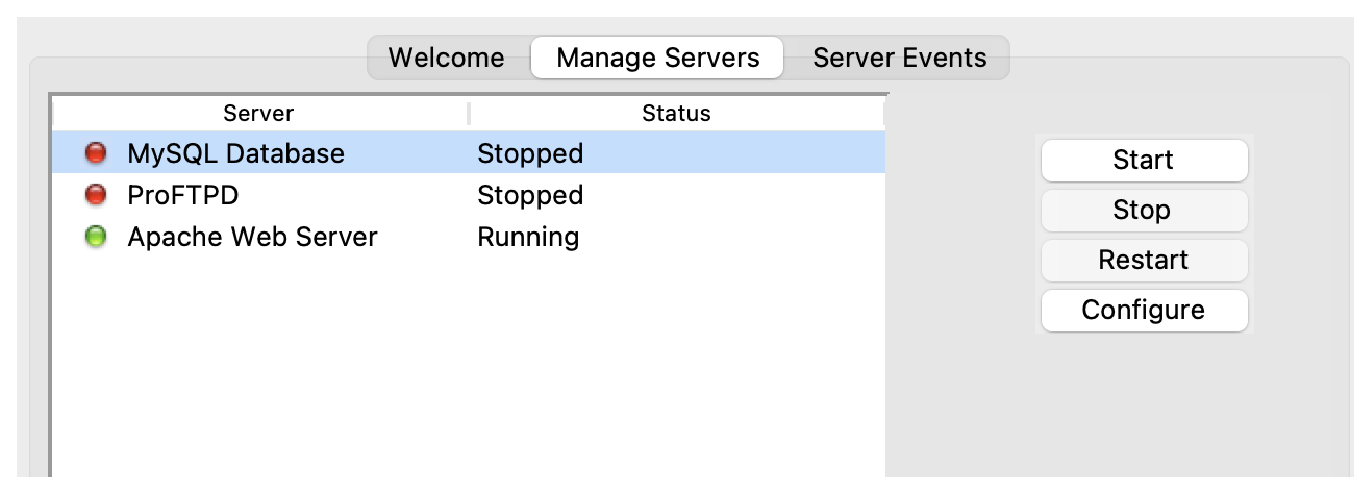
\includegraphics[width=70mm]{./fig/fig3.eps}
\caption{電子機器が外界から受ける妨害}
\label{fig3}
\end{figure}

\begin{table}[H]
\centering
\caption{イミュニティの例}
\label{table3}
\begin{tabular}{l|l} \hline
  \multicolumn{1}{c}{現象} & \multicolumn{1}{|c}{影響の例} \\ \hhline{=|=}
  \makecell[l]{電磁波} & \makecell[l]{テレビやオーディオへの雑音,\\コンピュータの誤動作,無線や有線の通信障害} \\ \hline
  \makecell[l]{電源やその他の導体を通して\\伝導する高周波ノイズ} & \makecell[l]{テレビやオーディオへの雑音,コンピュータの誤動作} \\ \hline
  \makecell[l]{静電気放電,サージ} & \makecell[l]{回路の誤動作や破壊} \\ \hline
  \makecell[l]{低周波磁界} & \makecell[l]{CRTの画像の歪み,ハム雑音} \\ \hline
  \makecell[l]{電源電圧変動や短時間の停電} & \makecell[l]{機器の機能停止や誤動作} \\ \hline
\end{tabular}
\end{table}

\subsection {EMCの達成について}
機器への干渉が問題となるのは,被害者となる危機が受ける妨害のレベルがその危機が耐えられる限界を超えた時になる.

\end{document}